\chapter{Apprentissage automatique et aide à la décision}

\section*{Introduction}

Depuis plusieurs années, l'apprentissage automatique est de plus en plus exploré
en vue de résoudre des problèmes complexes pour lesquels les statistiques
étaient impuissante. L'objectif de l'apprentissage automatique (machine
learning) est de réaliser des modèles qui apprennent des exemples.
Le machine Learning est un ensemble de méthodes qui permettent aux ordinateurs
d'apprendre à partir des données qui leurs sont soumises. Historiquement,
cette théorie a pris son essor avec les travaux des mathématiciens Vapnik et
Chervonenkis dans les années 60. Avec le Machine Learning, le point de vue est
différent de celui de la statistique traditionnelle. Les algorithmes d'apprentissage
automatique permettent aux ordinateurs de s'entraîner sur les entrées de données et 
utilisent l'analyse statistique pour produire des valeurs qui se situent dans une 
plage spécifique.


\section{Vocabulaire du machine learning}

\subsection{Etiquettes}
Une étiquette est le résultat de la prédiction ; la variable y dans une régression 
linéaire simple. Il peut s'agir du cours à venir du blé, de l'espèce animale représentée 
sur une photo ou de toute autre chose. 
Dans l'analyse d'un dossier, les étiquettes sont le résultat de l'analyse d'un
dossier.

\subsection{Caractéristiques}
Une caractéristique est une variable d'entrée ; la variable x dans une régression linéaire 
simple. Un projet de Machine Learning simple peut utiliser une seule caractéristique, 
tandis qu'un projet plus sophistiqué en utilisera plusieurs, spécifiées sous la forme :
$$
x1, x2, \ldots{}, x3
$$
\subsection{Exemples}
Un exemple est une instance de donnée particulière, x. Les exemples se répartissent dans deux
catégories : les exemples étiquetés et les exemples non-étiquetés.

\subsection{Modèles}
Un modèle définit la relation entre les caractéristiques$X$ et l'étiquette.
Par exemple, un modèle de détection de spam peut associer étroitement certaines
caractéristiques à du \og spam \fg.

Les principales étapes de la durée de vie d'un modèle sont les suivants:
\subsubsection{L'apprentissage}
L'apprentissage consiste à entraîner le modèle. En d'autres termes, il s'agit de
présenter au modèle des exemples étiquettés et de lui permettre d'apprendre
progressivement les relations entre les caractéristiques et l'étiquette.

\subsubsection{L'inférence}

L'inférence consiste à appliquer le modèle entraîné à des exemples sans
étiquette. Il s'agit  d'utiliser le modèle entrainé pour faire des prédictions
efficace.



%\input{sources/chapter3_ml/etape.tex}

\section{Les objectifs et méthodes du Machine learning}

Le choix de la méthode d'apprentissage dépend en grande partie de l'objectif
poursuivi.

\subsection{Les objectifs du machine learning}

Le machine learning poursuit plusieurs objectifs qui selon le cas peut être
 \subsubsection{Une classification}
Les modèles de classification prédisent des valeurs discrètes. Ils formulent, 
par exemple, des prédictions qui répondent à des questions telles que les suivantes:
\begin{itemize}
  \item Un e-mail donné est-il considéré comme du spam ou non?
  \item Cette image représente-t-elle un chien, un chat ou un hamster?
  \item Un dossier donné est-il conforme ou pas?
\end{itemize}

La classification est un processus en deux étapes, une étape 
d’apprentissage et une étape de prédiction, dans l’apprentissage machine.
Dans l’étape d’apprentissage, un modèle est développé à partir d’un 
ensemble de données préalablement étiquettés. Dans la phase de prédiction,
le modèle développé dans la phase précédente est utilisé pour prédire les 
étiquettes de nouvelles données.

\subsubsection{Une regression}
Les modèles de régression prédisent des valeurs continues. Ils formulent,
par exemple, des prédictions qui répondent à des questions telles que :
\begin{itemize}
  \item Quel est la valeur d'un logement au Burkina Faso ?
  \item Quel est la probabilité qu'un utilisateur clique sur cette annonce?
\end{itemize}

\subsubsection{Le clustering}
Le clustering est le regroupement d'exemples en classes d'objets similaires.
La différence entre clustering et classification est que les exemples sont
étiquetés dans une classification alors que dans le clustering, il ne le sont
pas.(Voir Figure \ref{fig:clustering})


\begin{figure}[h!]
  \begin{center}
    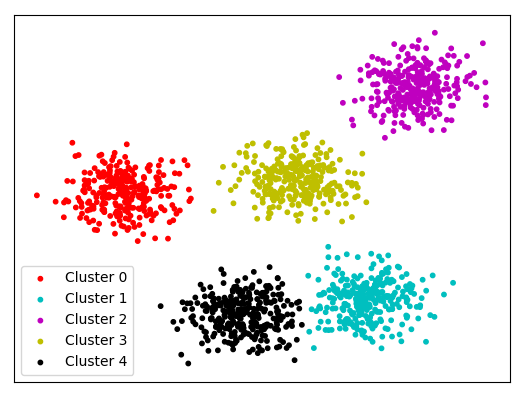
\includegraphics[width=14cm]{images/clustering.png}
      \caption{Clustering des données.\label{fig:clustering}}
  \end{center}
\end{figure}

Le but des algorithmes de clustering est de donner un sens aux données et
d'extraire de la valeur à partir de grandes quantités de données structurées ou
non-structurées. Ces algorithmes vont permettre de séparer les données en
fonction de leurs propriétés ou fonctionnalités et de les regrouper dans
différents clusters en fonction de leurs similitudes.




\subsection{Les méthodes d'aprentissage}
Les méthodes d'apprentissage automatique les
plus largement adoptées sont l'apprentissage supervisé et l'apprentissage
non-supervisé. Explorons donc ces méthodes plus en détail.

\subsubsection{L'apprentissage supervisé}
Le but de cette méthode est de permettre à l'algorithme  de découvrir 
l'étiquette réelle d'un exemple à partir des étiquettes apprises pendant la
phase d'entrainement, pour trouver des erreurs et modifier le modèle en 
conséquence. L'apprentissage supervisé utilise pour l'entrainement de son modèle,
des exemples étiquettés.

\subsubsection{L'apprentissage non-supervisé}
L’apprentissage non supervisé consiste à apprendre à classer sans supervision; les
exemples fournis sont non-étiquettés. L'objectif ici  est de réunir les 
exemples selon des critères prédéfinis par les équipes en charge du projet.En effet,
l’apprentissage non supervisé permet de regrouper des éléments non-classés dans 
différents groupes selon leurs caractéristiques.


\section{Les différents type de classifieurs}

Il existe plusieurs types de classifieurs. Nous présentons içi quelques
classifieurs avec leurs avantages et inconvénients.

 \subsection{Méthode des K plus proche voisins (KNN)}

La méthode des 'K plus proche voisins' ou \textbf{k-Nearest Neighbors
KNN} en \nomenclature{KNN}{K-Nearest Neighbors}
anglais est une méthode de classification dans laquelle le modèle mémorise 
les observations de l’ensemble d’apprentissage pour la classification des 
données de l’ensemble de test.\cite{pradaig}

Son fonctionnement peut être assimilé à l’analogie suivante:
\textit{dis moi qui sont tes voisins, je te dirais qui tu es}.
Pour effectuer une prédiction, l’algorithme \textbf{K-NN} ne va pas calculer
un modèle prédictif à partir d’un training set(ensemble d'apprentissage) comme c’est le cas pour la 
régression logistique ou la régression linéaire. C'est pourquoi cet 
algorithme est qualifié de paresseux (Lazy Learning) car il n’apprend
rien pendant la phase d’entrainement. 

\subsubsection{Prédiction avec K-NN}
K-NN se base sur le jeu de donnée entier pour effectuer une prédiction. Pour 
un exemple qu'on souhaite prédire qui ne fait pas parti du jeu de données \cite{datascientist}
initiale, l’algorithme va chercher les \textit{K} instances du jeu de données les 
plus proches de notre exemple. Ensuite pour ces \textit{K} voisins, l'algorithme
se basera sur leurs étiquettes pour calculer l'étiquette de l'exemple que l'on
souhaite prédire.(figure~\ref{fig:knnfonctionnement})

\subsubsection{Similarité dans l'algorithme K-NN}
K-NN a besoin d’une fonction de calcul de distance entre deux exemples. Plus 
deux points sont proches l’un de l’autre, plus ils sont similaires et vice 
versa\cite{nagesh2019}.

Il existe plusieurs fonctions de calcul de distance, notamment, la distance 
euclidienne, la distance de Manhattan, la distance de Minkowski, celle de 
Jaccard, la distance de Hamming \ldots. La fonction de distance se choisit en
fonction des types de données qu’on manipule. Ainsi pour des données 
quantitatives (poids, salaires, taille, montant de panier éléctronique\ldots),
la distance euclidienne est un bon candidat. Quant à la distance de Manhattan,
elle est une bonne mesure quand les données ne sont pas de 
même type (age, sexe, longueur, poids\ldots).

\begin{figure}[h!]
  \begin{center}
    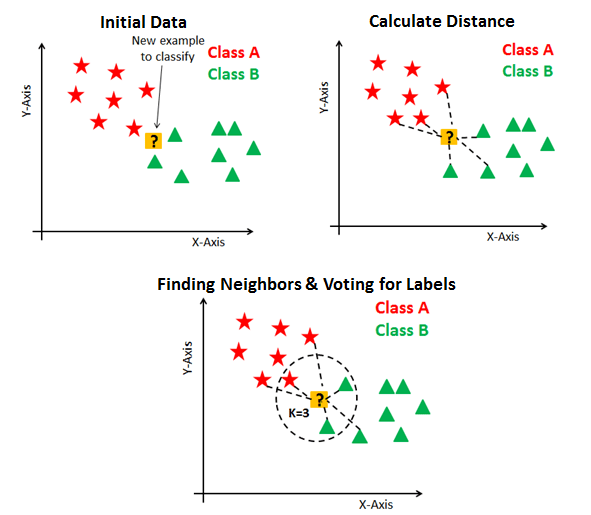
\includegraphics[width=12cm]{images/knn.png}
    \caption{Fonctionnement de l'algorithme K-NN.\label{fig:knnfonctionnement}}
  \end{center}
\end{figure}

\subsubsection{Choix de la valeur K}

Le choix de la valeur K varie en fonction du jeu de données. En règle générale, 
si K est petit, on sera sujet au sous apprentissage (underfitting). Par 
ailleurs, plus on utilise de voisins (K grand) la prédiction sera plus fiable. 
Toutefois, si on utilise K nombre de voisins avec K=N et N étant le nombre 
d’exemples, on risque d’avoir du overfitting et par conséquent un modèle qui se
généralise mal sur des observations qu’il n’a pas encore vu.

\subsubsection{Avantages}
\begin{description}
     \item{\textit{Absence d'apprentissage}}: Ce sont les échantillons pris en 
      considération, qui constituent le modèle.
    \item{\textit{Clarté des résultats: }} bien que la méthode ne produise pas de 
        règle explicite, la classe attribuée à un exemple peut être expliquée en
        exposant les plus proches voisins qui ont imposé cette attribution.
       \item{\textit{Grand nombre d'attributs:}} la méthode permet de traiter des
          problèmes avec un grand nombre d'attributs. Cependant, plus le nombre 
          d'attributs est important, plus le nombre d'exemples doit être grand.
      \end{description}

\subsubsection{Inconvénients}
\begin{description}
   \item{\textit{Sélection des attributs pertinents:}} Pour que la notion de proximité
    soit pertinente, il faut que les exemples couvrent bien l'espace et soient 
    suffisamment proches les uns des autres. Si le nombre d'attributs pertinents est
    faible relativement au nombre total d'attributs, la méthode donnera de mauvais 
    résultats.
   \item{\textit{Le temps de classification:}} Si la méthode ne nécessite pas 
    d'apprentissage, tous les calculs doivent être effectués lors de la classification 
    d'un nouvel exemple.
  \item{\textit{Définir les distances et nombres de voisins:}} Les performances de la 
      méthode dépendent du choix de la distance, du nombre de voisins et du mode de 
      combinaison des réponses des voisins.
  \end{description}

\subsection{Les réseaux de neurones}
Les réseaux de neurones sont inspirés de la structure neurophysiologique des
neurones. En règle générale, un réseau de neurones repose sur un grand nombre de
processeurs opérant en parallèle et organisés en tiers(couches). La première
couche reçoit les entrées d’informations brutes, un peu comme les nerfs optiques
de l’être humain lorsqu’il traite des signaux visuels. Par la suite, chaque
couche  reçoit les résultats de la couche précédente.
On retrouve le même processus chez l’Homme, lorsque les neurones reçoivent des
signaux en provenance des neurones proches du nerf optique. La dernière couche,
quant à elle, produit les résultats du système.

\subsubsection{Les différents cas d'usage}

Les réseaux de neurones sont beaucoup utilisés dans la reconnaissance d'écriture
manuscrites, la transcription \og speech-to-text \fg ou encore dans la
prévision des marchés financiers ou trading algorithmique.

Ils peuvent aussi être utilisé pour la reconnaissance faciale, la prédiction
météo, la détection de cancer sur les imageries médicales. De manière générale,
les réseaux de neurones excellent pour la reconnaissance de patterns.

\subsubsection{Avantages}
\begin{description}
  \item{\textit{Classification efficace :}} le calcul d'une sortie à partir d'un 
    vecteur d'entrée est un calcul très rapide.
  \item{\textit{Les données réelles :}} les réseaux traitent facilement les données 
      réelles "préalablement normalisées" et les algorithmes sont robustes au bruit.
  \end{description}

\subsubsection{Inconvénients}
\begin{itemize}
  \item Déterminer l’architecture du réseau est complexe et les
    paramètres sont difficiles à interpréter (boite noire).
    \item L'échantillon nécessaire à l'apprentissage doit être
      suffisamment grand et représentatif des sorties attendues.
  \end{itemize}

\subsection{Support Vector Machine (SVM)}
Les Support Vector Machine ou Machine à Vecteur de Support constituent une 
technique d’apprentissage supervisée. Elles ont été inventées par Boser, 
Guyon et Vapnik \cite{10.1145/130385.130401} et présentées pour la première
fois à la conférence Computational Learning Theory (COLT) de 1992.
Grâce à ses performances \cite{Cortes1995}, cette technique a ouvert un domaine de 
recherche très actif et un grand éventail d’applications. Les SVM utilisent
une approche géométrique pour classer les données en deux catégories.

En considérant les données comme des vecteurs, les SVM construisent un plan(une
frontière) qui sépare les données dans chacune des catégories.
Une fois la frontière de décision construite(Hyperplan) la
SVM\nomenclature{SVM}{Support Vector Machine} sera capable de
classer de nouvelles données en observant de quel côté de la frontière elles
tombent, et en leur assignant la catégorie correspondante.

L'idée est donc de rechercher le meilleur hyperplan qui sépare linéairement deux
classes, tout en les repoussant aux maximum. Lors de la phase d'apprentissage,
le svm cherche à maximiser la marge entre les deux classes d'apprentissage. Ce
qui lui procure une grande capacité de généralisation pendant la phase de test.

Les machines à vecteurs de support ont été appliquées dans des domaines comme
la reconnaissance automatique des visages et des gestes \cite{840634}, la
prédiction des mouvement de la bourse\ldots \cite{HUANG20052513}.

 Les domaines dans lesquels, elles sont les plus efficace sont: la reconnaissane d'objet et de
 d'image \cite{788125} et la catégorisation de texte \cite{6990940}



\begin{figure}[h!]
  \begin{center}
    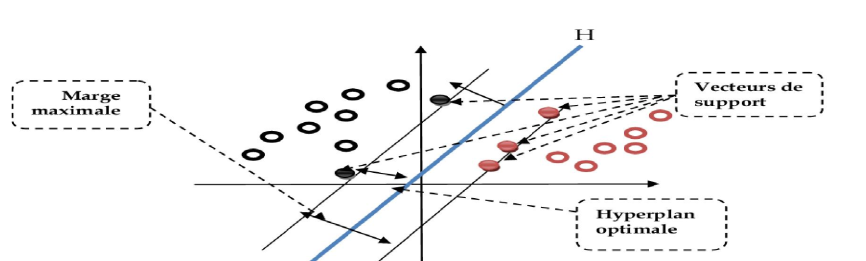
\includegraphics[width=14cm]{images/marge.png}
      \caption{Machine à vecteurs de support .\label{fig:marge}}
  \end{center}
\end{figure}

\subsubsection{Avantage}
\begin{itemize}
  \item Grâce à leurs fondements mathématiques solides, les SVM possèdent donc
    une grande précision de prédiction
  \item les SVM fonctionnent bien sur de petits jeux de données
  \item Décision rapide. La classification d’un nouvel exemple consiste à voir le signe de
    la fonction de décision f(x). 
\end{itemize}

\subsubsection{Inconvénient}
Les SVM ne conviennent pas à des jeux de données très volumineux car le temps
d'entrainement est très long.

  Les SVM effectuent une classification binaire d’où la nécessité d’utiliser 
l’approche un-contre-un pour construire un classifieur multiclasse.
Une grande quantité d’exemples en entrées implique un calcul matriciel important.
Le temps de calcul est élevé lors d’une régularisation des paramètres de la 
fonction noyau. 

Les SVM sont moins efficaces sur les jeux de données contenant
du bruits et beaucoup d’outliers

 \subsection{Les arbres de décisions}
Un arbre de décision est un outil d’aide à la décision qui permet de
répartir une population d’individus en groupes homogènes selon des attributs
discriminants en fonction d’un objectif fixé. Il permet d'émettre des
prédictions sur le problème par réduction niveau après niveau du domaine.

Les arbres de décision sont facilement interprétables, toutefois, leur capacité de
prédiction est presque toujours dépassée par les autres modèles de classication. 
Cette caractéristique a limité son utilisation. Au début des années 2000,
ils ont été repris comme élément de base d'une nouvelle méthode de
classification, appelée la forêt aléatoire de décision.

Cette nouvelle technique utilise de manière combinée les arbres de
décision et la théorie statistique pour réduire la variance du classeur en calculant la
moyenne d'un ensemble d'arbres de décision en générant des classeurs avec une très
bonne capacité de prévision. Nous les présenterons plus largement dans les
prochaines sections.

\subsubsection{Avantages}
\begin{description}
   \item{\textit{Adaptabilité aux attributs de valeurs manquantes :}} les
    algorithmes peuvent traiter les valeurs manquantes (exemples contenant
    des champs non renseignés) pour l'apprentissage, mais aussi pour la 
    classification.
  \item{\textit{Modèle white-box }} D'un arbre de décision, il
    est possible de générer des règles permettant d'expliquer ou de comprendre le
    résultat d'une classification. le résultat est facile à conceptualiser, 
    à visualiser et a interpréter.
  \item{\textit{Classification très rapide :}} Le coût d'utilisation des arbres est
    logarithmique.
  \item{\textit{Traitement de tous type de données: }} Les arbres de décisions
    prennent en compte aussi bien les échantillons ayant des caractéristiques
    continues que discrètes. Il est robuste au brruit.
  \item{\textit{Donne une classification efficace}} L'attribution d'une classe à
    l'aide d'un arbre de décision est obtenu grâce au parcours d'un chemin de
    l'arbre.
  \item{\textit{Ils ont un bon comportement par rapport aux valeurs extrêmes
    (outliers).}}
\end{description}

\subsubsection{Inconvénient}
  \begin{description}
     \item{\textit{Manque d’évolutivité dans le temps :}} Même si les données
      évoluent avec le temps, il est nécessaire de relancer une phase d'apprentissage 
      sur l'échantillon complet (anciens nouveaux exemples)
     \item{\textit{Méthode sensible au nombre de classes :}} les performances tendent à
      se dégrader lorsque le nombre de classes devient trop important.
    \item{\textit{Ils sont instables :}} D es changements légers dans les données produisent des 
      arbres très différents. Les changements des nœuds proches de la racine affectent 
      beaucoup l’arbre résultant. 
    \item{\textit{Sûr-apprentissage :}} Les arbres générés sont trop complexes et généralisent 
      mal (solution : élagage, contrôle de la profondeur de l’arbre et de la taille 
      des feuilles).
  \end{description}




\section{Comparaison des algorithmes de classification}

Le choix de l'algorithme optimal pour un problème donnée dépend de sa vitesse
d'entrainement et de prédiction, de la précision de ces prévisions, de la
quantité de données nécessaires à l'entrainement, de la facilité à la mettre en
oeuvre, et de la capacité à expliquer le résultat de la prédiction.

Le tableau ci-dessous présente une comparaison des différents algorithmes de
classification.

\begin{table}
  \begin{center}
    \renewcommand{\arraystretch}{1.5}

    \begin{tabular}{|c|c|c|c|c|c|}
      \hline
      \rowcolor[gray]{0.7}
      \bf\rule[-0.4cm]{0mm}{1cm} Algo & \bf Interprétabilite & \bf Précision & \bf{VE et VP} & \bf Données \\
      \hline
     \bf Knn & Oui & Faible & Dépend de K & Beaucoup \\
      \hline
     \bf Régression & Un peu & Faible & Rapide & Peu \\
      \hline
     \bf Naïves bayes & Un peu & Faible & Rapide & Peu \\
      \hline
     \bf Réseaux de neurones & non & Très élevé & Lent & Beaucoup \\
      \hline
      \bf{Arbre de décision} & Oui & Moyen & Rapide & Assez \\
      \hline
      \bf{Random Forest} & Non & Très élevé & Lent & Assez \\
      \hline
    \end{tabular}
    \caption{Tableau de comparaison des algorithmes de classifications}
    \label{tab:tab2}
  \end{center}
\end{table}
Le tableau \ref{tab:tab2} révèle que les algorithmes de Réseaux de neurones et ceux de forêt
aléatoire ont un taux très élevé de bonne prédiction. Malheureusement, ces
algorithmes fonctionnent bien sur des jeude données énormes. De plus la vitesse
d'apprentissage et de prédiction reste relativement lente par rapport aux
autres algorithmes.



\section{Les arbres de décisions}

Deux techniques de classification par les arbres ont été dévéloppées au
début des années 1980 par deux groupes de chercheurs.
Le premier groupe, dirigé par J Ross Quinlan, a développé un algorithme d'arbres
de décision en 1986 appelé ID3. Plus tard en améliorant plusieurs 
caractéristiques de ID3, il a développé et présenté C4.5.
L. Breiman, J. Friedman, R. Olshen, et C. Stone, un groupe de statisticiens, 
ont développé un algorithme pour produire des arbres de décision binaires 
appelé CART (Classication and Regression Trees) de leur côté. Ces algorithmes
ont été le début de la recherche sur la classification par les arbres de
décisions.  Les deux approches suivent le paradigme \og Diviser pour régner \fg

Plusieurs objectifs concourent à la construction d'un arbre de décision. Ce
sont:
\begin{itemize}
  \item Une meilleure généralisation des exemples de la base d'apprentissage.
  \item Une meilleure classification de nouveaux exemples
  \item Une structure aussi simple que possible
\end{itemize}
La construction d'un arbre de décision consiste à partitionner un ensemble de 
données en des groupes les plus homogènes possible du point de vue de la 
variable à prédire. On prend en entrée un ensemble de données classées, et on 
fournit en sortie un arbre. Nous obtenons un arbre qui représente une série de 
noeuds en plaçant dans la partie supérieure le noeud dont la capacité de 
classification est la plus grande. \cite{criminisi2011} 
Le résultat final est un arbre renversé comme celui représenté dans la figure
\ref{fig:DecisionTree}

\begin{figure}[h!]
  \begin{center}
    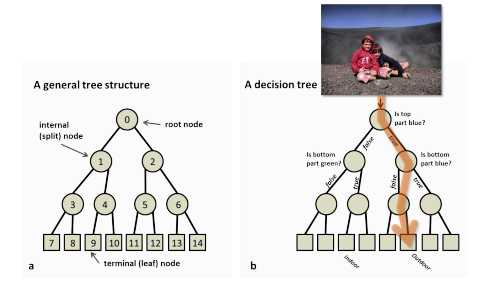
\includegraphics[width=14cm]{images/decisionTree.png}
    \caption{Arbre de décision. 
	\label{fig:DecisionTree}}
  \end{center}
  \textit{Le $a$ représente la structure générale d'un arbre de décision. Le
$b$ montre un arbre de décision illustratif utilisé pour déterminer 
si une photo représente une scène d'intérieur ou d'extérieur.}
\end{figure}

\subsection{Structure d'un arbre de décision}

Le fonctionnement des arbres de décisions repose sur les heuristiques 
construites sur des techniques d'apprentissage supervisées.

Les arbres de décisions sont composés de noeuds et de feuilles reliés par des
branches. Dans leur représentation graphique la raçine est placée tout en haut
et les feuilles en bas. Les noeuds internes sont appelés des noeuds de décision.
Ils peuvent contenir une ou plusieurs règles. Les noeuds terminaux contiennent
la classe aussi appelée classe à prédire ou étiquette. Après sa construction, un
arbre de décision peut être traduit par un ensemble de règle.

L'algorithme  générique  de construction d'un arbre permet de générer
itérativement l'arbre en prenant à chaque itération une variable et en lui
créant ses noeuds et ses feuilles. L'idée centrale est la suivante:

\textit{Diviser récursivement et le plus efficacement possible les exemples de  
l'ensemble d'apprentissage par des tests définis à l'aide des attributs
jusqu'à ce que l'on obtienne des sous-ensembles d'exemples ne contenant 
(presque) que des exemples ayant tous la même étiquette.}

 \subsection{Optimisation des noeuds}
 
 En général, on décide qu'un noeud est terminal lorsque tous les exemples
 associés à ce noeud, ou du moins  la plupart d'entre eux ont la même étiquette
 ou s'il n'y a plus d'autres caractéristiques non utilisées dans la branche
 correspondante.

 La sélection d'un test à associer à un noeud pour obtenir un arbre optimal 
 est un choix crucial. En effet, construire un arbre de décision optimal
 consiste à construire un arbre de décision le plus petit possible rendant compte
 au mieux des données. Il s'agit donc de rechercher le test qui permet de faire
 évoluer la tâche de classification. Pour mesurer cette évolution, \textit{CART}
 utilise l'\textit{indice de Gini}. Les algorithmes de Quinlan eux, utilisent  la
 notion d'\textit{entropie}.

 \subsubsection{Entropie de Shannon}

L'entropie de Shannnon correspond à la quantité d'information fournies par un
évènement: plus la probabilité d’un événement est faible (il est rare), plus 
la quantité d’information qu’il apporte est grande. Sa formule est la
suivante
\cite{benjamin2005}:
$$  
Entropie = - \sum_{i=1}^{n} {p_i * log_2(p_i)}
$$ 
Tel que $p_i$ est la proportion d'exemples de S ayant pour classe résultante
(étiquette) $i$. 

Pour un ensemble de données $T$ caractérisé par $n$ classes ($C_1, C_2, \cdots,
C_n$) selon la variable cible, la quantité d'information nécessaire pour
identifier la classe d'un individu correspond à l'entropie $E(P)$ où $P$est la
distribution de probabilité de la partition ($C_1, C_2, \cdots, C_n$).
$$
P = (\frac{|C_1|}{|T|}, \frac{|C_2|}{|T|}, \cdots, \frac{|C_n|}{|T|})
$$
$|C_i|$ représente le cardinal de la classe $i$ c'est-à-dire le nombre
d'éléments de la classe $i$.

L'entropie de $T$ est alors:

$$
Entropie(T) = - \sum_{i=1}^{n}{\frac{|C_i|}{|T|} log_2\frac{|C_i|}{|T|}}
$$

La fonction permettant de sélectionner le test qui doit étiqueter le noeud
courant  est la fonction \textit{Gain}. Pour un ensemble de données $T$, le gain
d'information de $T$ par rapport à une partition $T_j$ donnée est la variation
d'entropie causée par la partition de T selon $T_j$
$$
Gain(X, T) = Entropie(T) - Entropie(X, T) = Entropie(T) - \sum_{j=1}^{m} {\frac{T_j}{T} * Entropie(T_j)}
$$

Le gain permet de calculer ce que l'attribut spécifié apporte au désordre
du set. Plus un attribut contribue au désordre, plus il est important de le
tester pour séparer le set en plus petits sets ayant une entropie moins 
élevée.

\subsubsection{Indice de Gini}
L'indice de Gini est une mesure statistique permettant de rendre compte de la
répartition d'une variable au sein d'une population. Il mesure l'impureté qui
est un concept très utile dans la construction des arbres de décision: La qualité
d'un noeud et son pouvoir discriminant peuvent être évalués par son impureté.
Sa formule est la suivante:
$$
Gini(T) = 1 - \sum_{j=1}^{m}{(p_i)^2} =  1 - \sum_{j=1}^{m}{(\frac{|T_j|}{|T|})^2} 
$$




\subsection{Algorithmes d’induction d’arbres de décision}

Il existe essentiellement deux grandes familles d'algorithmes permettant de construire
des arbres de  décisions à partir d'un set de données: les algorithmes de
Quinlan (\textbf{ID3}, \textbf{C4.5}, \textbf{C5.0}) et l'algorithme
\textbf{CART}. Les deux approches suivent le paradigme \og diviser pour régner
\fg. Nous présentons ici le principe des trois algorithmes de construction des
arbres de décision que sont l'algorithme ID3, l'algorithme C4.5 et l'algorithme
CART.

%\input{sources/chapter4_arbre/generic}

   \subsubsection{CART}
  L'algorithme Classification and Regression Trees(\textit{CART}) est très
  similaire à C4.5, mais il en diffère par le fait qu’il prend en charge la
  régression en ne calculant pas des ensembles de règles. Il s'agit d'un  
  algorithme développé par Breiman, Friedman, Olshen et Stone (1984).

  Selon l'algorithme CART, un arbre de décision est construit en déterminant
  les questions (appelées fractionnements de noeuds) qui, lorsqu'on y répond,
  conduisent à la plus grande réduction de l'impureté de Gini. Cela signifie 
  que l'arbre de décision tente de former des noeuds contenant une forte 
  proportion d'échantillons (points de données) provenant d'une seule classe en
  trouvant des valeurs dans les caractéristiques qui divisent proprement les 
  données en classes(étiquettes).
 
  \subsubsection{ID3}
  Iterative Dichotomiser 3(\textit{ID3}) a été developpé par Ross Quinlan en
  1986. Il se base qur le concept d'attribut et de classe. L'algorithme 
  recherche l'attribut le plus pertinent à tester pour que l'arbre soit le
  plus court et le plus optimisé possible en déterminant l'attribut qui
  maximise le gain d'information.\cite{quinlaninduction}

  L'algorithme crée un arbre multivoie, trouvant pour chaque nœud (c'est-à-dire
  de manière gourmande) la caractéristique catégorielle qui produira le plus 
  grand gain d'informations pour les cibles catégorielles. Les arbres sont 
  cultivés jusqu'à leur taille maximale, puis une étape d'élagage est 
  généralement appliquée pour améliorer la capacité de l'arbre à généraliser 
  les données invisibles.

  \subsubsection{C4.5}
 L’algorithme \textit{C4.5} est une évolution de l’algorithme ID3. Il a 
 également été inventé par Ross Quinlan. Basé sur ID3, C4.5 possède quelques
 améliorations\cite{quinlanc45}
  \begin{itemize}
    \item Une adaptation de la fonction gain qui n'a plus tendance à aller vers
     l'attribut avec le plus de valeur possible.
    \item La possibilité de gérer les valeurs manquantes.
    \item La possibilité de post-élaguer son arbre pour éviter l'overfitting;
    \item La possibilité de manipuler des valeur continues
  \end{itemize}
  \textit{C5.0} est la dernière version de Quinlan publiée sous une licence 
  propriétaire. Elle utilise moins de mémoire et construit des jeux de règles 
  plus petits que C4.5 tout en étant plus précise.


  \begin{table}
    \begin{center}
       \renewcommand{\arraystretch}{1.5}
  \begin{tabular}{|l|c|c|}
    
    \hline
    \rowcolor[gray]{0.7}
     \renewcommand{\arraystretch}{1.5}\bf Méthode & \bf CART & \bf C4.5 \\
    \hline
    \bf{Mesure utilisé pour la sélection} & index Gini & Entropie et Gain d'info \\
    \hline
    \bf{Type des variables(attributs)} & discrètes et continues & discrètes et
    continues \\
    \hline
    \bf{Division à chaque noeud} & binaire & multiple \\
    \hline
   \end{tabular}
   \caption{Tableau comparatif des algorithmes C4.5 et CART}
    \label{tab:tab1}
  \end{center}
\end{table}



Dans le cadre de notre projet, l'algorithme qui sera utilisé pour la génération
de notre arbre de décision est \textit{C4.5}. Il permet la manipulation  de
valeurs continues et ne génère pas un arbre de décision binaire comme
\textit{CART} (tableau \ref{tab:tab1}).


Un modèle flexible  mémorise essentiellement les données d'entrainement en
les ajustant étroitement. Le problème d'un tel modèle est qu'il apprend non
seulement les relations réelles dans les données d'entrainement , mais aussi
tout bruit présent dans ces données. Un modèle rigide est dit avoir un biais
élevé parce qu’il fait des hypothèses sur les données de formation. Par
exemple, un classifieur linéaire fait l'hypothèse que les données sont linéaires
et n'a pas de flexibilité pour s'adapter à des données non linéaires.

Dans les deux cas (modèle flexible et modèle rigide), le modèle n'est pas capable de
réaliser de bonnes prédictions sur de nouvelles données.
Les arbres de décisions sont des modèles d'apprentissage flexible donc
sensible au bruit. Ils peuvent devenir très profonds c'est à dire croître
jusqu'à ce qu'il ait exactement une feuille pour chaque observation, les
classant toutes parfaitement.

Comme alternative, la forêt aléatoire empêche ce phénomne en créant des
sous-ensembles aléatoires des caractéristiques et en construisant des arbres plus
petits à l'aide de ces sous ensembles. Dans la suite nous présenterons les
forêts aléatoires une méthode supervisée d'apprentissage machine.

\section{Les forêts aléatoires}

  La forêt aléatoire est un modèle composé de nombreux arbres de décision. Plutôt
  que de se contenter de faire la moyenne des prédictions des arbres (que nous 
  pourrions appeler une \og forêt\fg), ce modèle utilise deux concepts clés qui lui 
  donnent le nom d'aléatoire:
  \begin{itemize}
    \item L'échantillonage aléatoire des données d'entrainement lors de la
      construction de l'arbre.
    \item Des sous-ensembles aléatoires de caractéristiques pour le fractionnement
      des noeuds
  \end{itemize}
  L’algorithme effectue un apprentissage en parallèle sur de multiples arbres
  de décision construits aléatoirement et entraînés sur des sous-ensembles de
  données différents. Le nombre idéal d’arbres, qui peut aller jusqu’à 
  plusieurs centaines voire plus, est un paramètre important : il est très 
  variable et dépend du problème.

  \subsection{Fonctionnement des forêts aléatoires}

  La forêt aléaoire (Random Forest) fonctionneen deux phases. La première
  consiste à créer la forêt aléatoire en combinant $N$ arbres de décisions. La
  seconde consisteà faire des prédictions pour chaque arbre créé dans la
  première phase.

  Le processus peut être expliqué dans les étapes ci-dessous:
  \begin{description}
    \item[Etape 1:] Sélectionnez k instances dans l'ensemble
      d'apprentissage.
    \item[Etape 2:] Construire les arbres de décisions associés aux points de
      données sélectionnés.
    \item[Etape 3:] Répétez les étapes 1 et 2, $N$ fois. ($N$ étant le nombre d'arbres
      de la forêt)
    \item[Etape 4:]Pour une nouvelle instance de données, trouvez la
      prédiction de chaque arbre de décision de la forêt et attribuez
      l'étiquette qui remporte la majorité des votes.
  \end{description}

  Supposons qu'il existe un ensemble de données contenant plusieurs images de
  fruits. Cet ensemble de données est attribué à un modèle de forêt aléatoire.
  L'ensemble des données est alors divisé en sous-ensemble et donné à chaque
  arbre de décision. Pendant la phase d'apprentissage, chaque arbre de décision
  produit résultat de prédiction. Lorsqu'une nouvelle instance apparaît, le
  modèle prédit la décision finale.

  \begin{figure}[h!]
    \begin{center}
      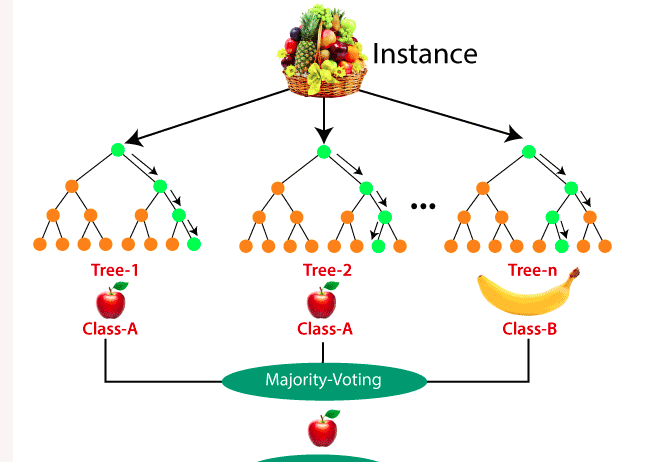
\includegraphics[width=14cm]{images/foret.png}
      \caption{Forêt aléatoire.\label{fig:foretaleatoire}}
    \end{center}
  \end{figure}


   \subsubsection{Echantillonage aléatoire des données d'entrainement}

    Lors de la phase d'entrainement, chaque arbre d'une forêt aléatoire apprend
    à partir d'un échantillon aléatoire de données. Les échantillons sont tirés 
    avec remplacement, connu sous le nom de \og bootstrapping \fg, ce qui 
    signifie que certains échantillons seront utilisés plusieurs fois dans un 
    seul arbre.

    Les prédictions sont faites en faisant la moyenne des prédictions de chaque
    arbre de décision. Cette procédure est connue sous le nom de \textit{bagging}
    abbréviation de \textit{bootstrap aggregating}

   \subsubsection{Fractionnement des noeuds}

    Le deuxième concept principal de la forêt aléatoire est que seulement un
    sous-ensemble de toutes les caractéristiques est pris en compte pour 
    diviser chaque noeud d'un arbre de décision. Cette valeur est 
    habituellement la raçine carré du nombre de caractéristiques pour une
    classification. Ainsi si nous avons 25 caractéristiques seulement 5
    seront pris aléatoirment pour diviser le noeud.

  \subsection{Les hyperparamètres dans les forêts aléatoires}

  Les hyperparamètres de la forêt aléatoires sont utilisés pour augmenter le
  pouvoir prédictif du modèle, soit pour rendre le modèle plus rapide.

  \subsubsection{Augmenter le pouvoir prédictif du modèle}

  Plusieurs hyperparamètres permettent d'augmenter le pouvoir de prédiction du
  modèle;
  \begin{description}
    \item[n\_estimators: ]Il s'agit du nombres d'arbres que l'algorithme
      construit avant de prendre le vote maximum ou la moyenne des prédictions.
      En général, un nombre d'arbres élevé augmente la performance et rend les
      prédictions plus stables mais ralentit également le calcul.
    \item[max\_features: ]Il s'agit du nombre maximum de caractéristiques qu'une
      forêt aléatoire considère pour diviser un noeud.
    \item[min\_sample\_leaf: ] Il s'agit du nombre minimum de feuilles nécessaires
      pour diviser un noeud interne.
  \end{description}

  \subsubsection{Augmenter la vitesse d'exécution du modèle}

  Les hyperparamètres permettant d'accélérer le modèle sont les suivants:
  \begin{description}
    \item[n\_jobs: ] Il indique au moteur le nombre de processeurs qu'il est autorisé
      à utiliser. Une valeur de $-1$ signifie qu'il n'y a aucune limite sur le
      nombre.
    \item[random\_state: ] Il rend la sortie du modèle reproductible. Le modèle
      produira toujours les mêmes résultats si on lui donne les mêmes
      hyperparamètres et les mêmes données d'entrainement.
    \item[oob\_score: ] Il s'agit d'une méthode de validation croisée des forêts
      aléatoires. Dans cette échantillonage, environ un tiers des données n'est
      pas utilisé pour entrainer le modèle mais plutôt pour évaluer ses
      performances sans aucune charge de calcul supplémentaire.
  \end{description}


\subsection{Les avantages et les inconvénients du modèle des forêts aléatoire}

\subsubsection{Avantages}
\begin{itemize}
  \item Les forêts aléatoires permettent de surmonter le problème de
    sur-ajustement en faisant la moyenne ou en combinant les résultats de
    diffrents arbres de décisions.
  \item Les forêts aléatoires fonctionnent mieux sur un large éventail de
    données qu'un seul arbre de décision.
  \item Les forêts aléatoires présentent moins de variance qu'un arbre de
    décision unique
  \item Les forêts aléatoires possèdent une très grande précision.
  \item Les algorithmes de forêt aléatoire maintiennent une bonne prédiction
    même si certaines informations sont absentes.
\end{itemize}

\subsubsection{Inconvénients}
\begin{itemize}
  \item La complexité est le principal inconvénient des algorithmes de Random
    Forest.
  \item La construction de forêts aléatoires est beaucoup plus
    difficile et longue que celle des arbres de décision.
  \item Il faut davantage de ressources de calcul pour mettre en oeuvre
    un algorithme de forêt aléatoire.
  \item Il est moins intuitif dans le cas où nous disposons d'une grande
    collection d'arbres de décision.
  \item Le processus de prédiction utilisant les forêts aléatoires est très long
    par rapport aux autres algorithmes.
\end{itemize}





\section*{Conclusion}

Ce chapitre nous a permis de présenter le machine learning et quelques algorithmes 
de classifications. En outre, nous nous sommes attardés sur les arbres de décisions 
qui sont un type de classifieurs qui nous pensons sont adaptés au contexte de notre étude.
Maintenant, nous poursuivrons en  présentent la conformité dans le domaine bancaire.
